\section{Miglioramento delle prestazioni: i delegati}
TensorFlow Lite mette a disposizione diverse strategie per l’ottimizzazione e la massimizzazione delle prestazioni di un modello di machine learning.
Uno di questi è il delegato. Un delegato consente di eseguire i modelli (in parte o interamente) su un altro esecutore più efficiente specificatamente
per il tipo di modello e la piattaforma su cui si esegue.                                                                                                                                       

I delegati abilitano l'accelerazione hardware dei modelli TensorFlow Lite sfruttando gli acceleratori sul dispositivo come la GPU e il processore di
segnale digitale (DSP).

Come impostazione di default TensorFlow Lite utilizza kernel CPU per l’ottimizzazione del set di istruzioni ARM Neon. Tuttavia, la CPU non è
necessariamente ottima per l'aritmetica complessa tipica dei modelli di machine learning. La maggior parte dei telefoni cellulari attuali contiene,
però, chip che sono in grado di gestire meglio queste operazioni pesanti. Utilizzarli per le operazioni di rete neurale offre enormi vantaggi in termini
di latenza ed efficienza energetica. Per esempio, le GPU riescono a velocizzare fino a 5 volte la latenza, mentre il processore DSP è in grado di ridurre
del 75\% il consumo di energia. A ciascuno di questi acceleratori sono associate API che consentono la computazione personalizzata, come OpenCL o OpenGL
ES per GPU e Hexagon SDK per DSP. Dunque, per il corretto funzionamento degli acceleratori è necessario scrivere parecchio codice. TensorFlow Lite risolve
il problema fornendo delle API che fungono come ponte tra il runtime TFLite e queste API di basso livello.

\begin{figure}[ht]
    \centering
    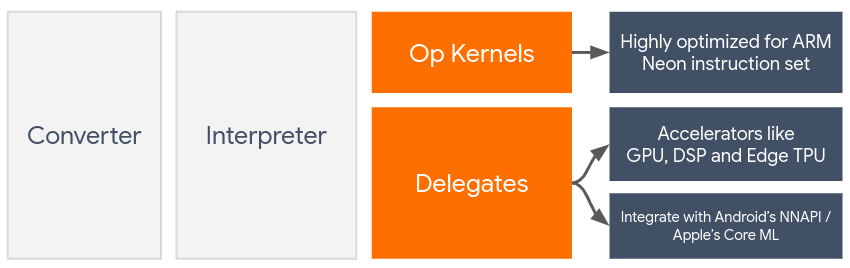
\includegraphics[width=0.8\textwidth]{Immagini/delegate_runtime.png}
    \caption{Distinzione tra kernel CPU e i delegati.}
    \label{fig:distinzione}
\end{figure}

\subsection{Scelta di un delegato}
TensorFlow Lite supporta più tipi di delegati, ognuno dei quali è ottimizzato per determinate piattaforme e particolari modelli. Nello specifico,
la scelta di un delegato si basa su due criteri principali: la piattaforma (Android o iOS) e il tipo di modello (a virgola mobile o quantizzato) da
accelerare. Per quanto riguarda la piattaforma:
\begin{itemize}
    \item Multipiattaforma (Android e iOS): GPU è l’unico tra i vari delegati che permette l’utilizzo sia su android che su iOS;
    \item Android: Ci sono due delegati che supportano l’utilizzo su android (e NON su iOS), ossia il delegato NNAPI (disponibile in android 8.1 e
    versioni successive) e il delegato Hexagon (disponibile in versioni android precedenti che non supportano NNAPI);
    \item iOS: L’unico delegato ottimizzato per iOS è Core ML (disponibile su dispositivi mobili apple con SoC A12 o superiore).
\end{itemize}
Per quanto riguarda il tipo di modello:
\begin{center}
    \begin{tabular}{ |c|c|c|c|c| }
        \hline
        \textbf{Tipo di modello} & \textbf{GPU} & \textbf{NNAPI} & \textbf{Hexagon} & \textbf{CoreML} \\
        \hline
        Virgola mobile (32 bit) & \checkmark  & \checkmark & X & \checkmark \\
        \hline
        Quantizzazione float16 post-training & \checkmark & X & X & \checkmark \\
        \hline
        Quantizzazione della gamma dinamica post-training & \checkmark & \checkmark & X & X \\
        \hline
        Quantizzazione intera post-training & \checkmark & \checkmark & \checkmark & X \\
        \hline
        Training consapevole della quantizzazione & \checkmark & \checkmark & \checkmark & X \\
        \hline
        
    \end{tabular}
\end{center}

Ogni acceleratore è progettato per una certa larghezza di bit dei dati. Per esempio, se viene fornito un modello in virgola mobile ad un delegato che
supporta solo operazioni quantizzate a 8 bit (come il delegato Hexagon), allora il delegato non accetterà il modello il quale verrà eseguito interamente
sulla CPU.

Scegliere la configurazione di accelerazione hardware ottimale per il dispositivo di ciascun utente può essere difficile. Inoltre, abilitare la
configurazione errata su un dispositivo può causare elevata latenza, errori di runtime o problemi di precisione causati da incompatibilità hardware
sfociando, quindi, in un servizio scadente e insoddisfacente per l’utente. In questo contesto, TensorFlow Lite mette a disposizione un \textbf{servizio di
accelerazione per Android}: un'API che aiuta nella scelta della configurazione di accelerazione hardware ottimale per un determinato dispositivo utente e
per uno specifico modello, riducendo al minimo il rischio di errori di runtime o problemi di precisione.

Il servizio di accelerazione valuta diverse configurazioni di accelerazione sui dispositivi target eseguendo benchmark di inferenza con il modello
TensorFlow Lite creato. I risultati dell’esecuzione dei benchmark possono essere salvati su cache e utilizzati durante l’inferenza. Inoltre, questi
benchmark sono fuori processo, riducendo al minimo il rischio di arresti anomali dell’applicazione Android.

\begin{figure}[ht]
    \centering
    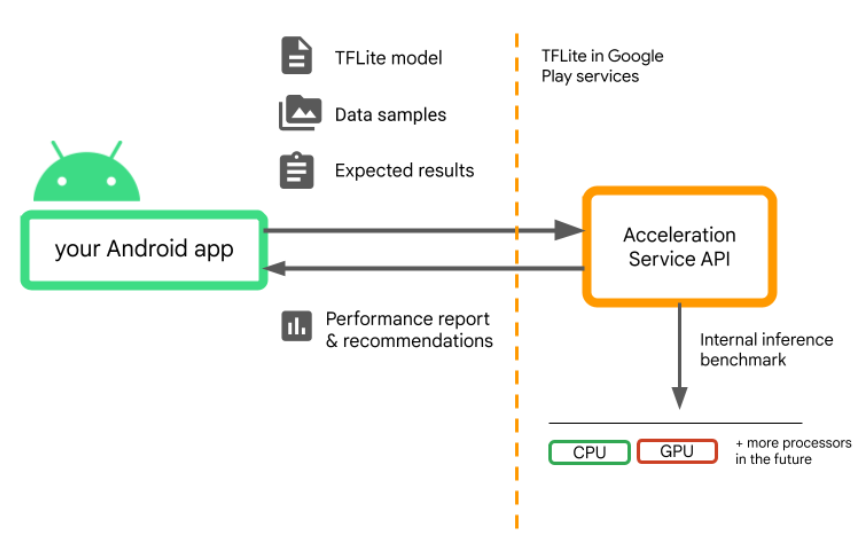
\includegraphics[width=0.7\textwidth]{Immagini/accelerazione.png}
    \caption{Schema riassuntivo del funzionamento del servizio di accelerazione}
    \label{fig:accelerazione}
\end{figure}

Fornendo il  modello, i campioni di dati e i risultati attesi il servizio di accelerazione eseguirà un benchmark di inferenza TFLite per fornire
consigli hardware allo sviluppatore.

\subsection{Tools per la valutazione}
TensorFlow Lite fornisce strumenti di valutazione delle prestazioni e dell’accuratezza che consentono agli sviluppatori di analizzare e verificare
l’efficienza dell’utilizzo dei delegati nell’applicazione creata. I due principali tools utilizzati sono:
\begin{itemize}
    \item Tools per la latenza e l’utilizzo di memoria: che stimano le prestazioni del modello considerando la latenza media di inferenza,
    l’overhead di inizializzazione, l’ingombro di memoria e altri;
    \item Tools per l’accuratezza e la correttezza: tendenzialmente, i delegati eseguono calcoli con una precisione differente rispetto ai kernel CPU.
    Di conseguenza, quando uso un delegato per l’accelerazione hardware la precisione tende a diminuire. Questo non succede sempre: per esempio la GPU,
    che esegue operazioni in virgola mobile, potrebbe migliorare leggermente la precisione. I tools che misurano questa metrica possono essere basati o
    meno sulla task specifica da valutare.
\end{itemize}